\chapter{Evaluation of Existing Applications}
\label{chp:3:EvalExisAppl}
After building the foundation on related work on personalized mass email communication, this section will evaluate existing systems available in the market. 

\section{Application Categories and Their Relation with The Thesis}
\label{sec:3.1:SystCate}

There are three different application categories that are related with this thesis, and focusing on email communication directly or indirectly. Followings section will give a brief description of those are these product types, and their relation with this thesis:

\subsection{Customer Relationship Management (CRM)}
\label{subsec:3.1.1:Cust}
A \ac{CRM} application helps to manage customer relationships effectively, which is a topic studied both by academia and industry in recent years. Such applications play an important role in the marketing where organizations use more customer oriented instead of product or brand oriented marketing strategies. Therefore, each customer's economic value is different to the company, and organizations' customer relation strategies require to adapt their customer offerings and communication strategy personalized according to individual customer \citep{Reinartz2004}. 
\vspace{1cm}

One of the reason why this thesis considers \ac{CRM} applications to evaluate is its communication aspects of a company with their clients. Another reason is, as it is mentioned at section 2.3, the adequate amount of personalization in emails is crucial on response rates, and people's increased daily interactions with digital world make the true authentic personalization more rare. To achieve such a level of personalization requires getting know each recipient very well by considering not only the recent conversation, but also earlier conversations, and all the information that might be extracted from those conversations helping to build a relation with respondents. Since a \ac{CRM} system aims to keep track of each customer history regarding a product or a brand, such a data store could be leveraged to add adequate amount of personalized information to a email conversation. 

\subsection{Help Desk}
\label{subsec:3.1.2:HelpDeskSoft}
Another application that focuses on a company and its relation with their clients is help desk applications. It's main purpose to provide information and support related to a company's products and services to their customers. As a part of knowledge acquisition, help desks supports both sides of the communication in a way that while customers or end users find the knowledge they need, and the people who provide help by making the knowledge available and reusable \citep{Halverson2004}.
\vspace{1cm}

Reusing the existing knowledge requires to structure the captured knowledge. This is where it makes the relation with this thesis. Because, a help desk application provides a workflow where both parties develop a communication where person who needs assistance describes his/her problem while people who provide help identify the problem by looking earlier cases or asking questions to clarify the initial question. This also requires the cooperation of assistants while providing help to a problem at which one person might have previous experience to guide other assistants. As a result, a help desk application is similar to a mass email communication where a researcher initiate an open ended questionnaire, extracting information from the coming replies, and organize them according to the answers that researcher seeks for. In addition, respondents might also come up with some questions to clarify things, where existing answers can easily be reused. Having such a email conversation with large groups require great amount of effort from a researcher's side, where he might assign tasks to distribute the efforts to other researchers to deal with the large size of the group.


\subsection{Email Marketing}
\label{subsec:3.1.3:EmaiMarkt}
Organizations and marketers use email marketing for several reasons. Some of those purposes are brand and customer loyalty building, acquiring or converting customers, advertising the brand or the product, solicit sales or donation, communicating for promotional offers and even educational purposes. At the end, these approaches can be group under following categories \cite{Eley2009}:

\begin{compactitem}
	\item \textbf{Educational Communication:} An educational message is given in the form of newsletter, avoiding sale push, but it might still consists some content indirectly by encouraging recipients. For example, free monthly newsletter which contains tips about digital photography, and photography accessories used in the tips might be linked to an online shopping website. 
	\item \textbf{News and Updates:} To notify the customers about important updates or changes to a business. For instance, release of a new product, changes on contact details or major changes on a company's website
	\item \textbf{Direct Sales Messages:} Emails sent by others consists marketing ads, and clear message on offers.
	\item \textbf{Housekeeping:} Emails such as subscription confirmation messages or welcome emails. These messages are often system generated automated messages. However, they can be used to promote a message as well like offering a discount code a long with the registration confirmation email.
\end{compactitem}

Since these categories consists communication with large group of people, this thesis also evaluates existing tools in the market for email marketing including its technical aspects.

\section{Methodology}
\label{sec:3.2:Meth}

The analysis examined two products from the categories of \ac{CRM}, help desk, and email marketing. Selection of the products depends on the several product comparison websites including Toptenreviews.com\footnote{http://\{email-marketing-software-review, crm-software-review\}.toptenreviews.com/ }, Softwareshortlist.com\footnote{http://www.softwareshortlist.com/crm/solutions/}, as well as from the suggestions of Stanford HCI group members\footnote{http://hci.stanford.edu/people/}. In addition to those websites and suggestions, their demo or trial version availability were also considered, since some of the products required fee before using them. After the products were shortlisted, the last filtering was done by getting their web traffic rankings from Compete.com\footnote{https://www.compete.com/}, Alexa\footnote{http://www.alexa.com/}, and Google Trends\footnote{http://www.google.com/trends/}. Finally, trial accounts were created on those application, and a scenario is simulated to get the full insight from them. 

\section{Results}
\label{sec:3.3:Resul}
Evaluation of the products will be done according to their category. A brief description of the products will be presented. This description will mainly focus on the features which are related to support email communication as explained in section~\ref{sec:3.1:SystCate}. After that each category will be concluded with a comparison matrix of the selected products.

\subsection{CRM Applications}
\label{subsec:3.3.1:CRMAppl}

\begin{table}[!ht]
\begin{center}
	%\renewcommand{\arraystretch}{2}
	%\tiny
	%\setlength{\tabcolsep}{5pt}
	\caption[Comparison Matrix for CRM Applications]{Comparison Matrix for CRM Applications} \label{tab:comp_matr_crm}
    \begin{tabular}{ p{3cm} p{3cm}  p{3cm} }
	\hline
	& \textbf{SugarCRM} & \textbf{Highrise} \\ \hline
	\textbf{Neutral power} & 143 (40.1) & 158 (44.4) \\
	\textbf{High power} & 150 (42.1) & 154 (43.3) \\ \hline
    \end{tabular}
\end{center}
\end{table}

\paragraph{SugarCRM}
SugerCRM comes in three different deployment versions. These are on-premise, \ac{SaaS}, and the free community edition. It has a clean \ac{UI} with a single navigation menu. Its calendar view can be synchronized with Outlook's calendar or any platform which supports iCalendar\footnote{iCalendar is the calendar data exchange stanard (RFC 5545) having file extension of .ics, and it allows sending meeting requests or tasks via email.}. It provides email management right in the application, and integrates with several platform like Outlook and Gmail or an \ac{IMAP} based email server. Users can archive emails in the SugarCRM by adding a unique email address into TO, \ac{CC}, or \ac{BCC} fields. This address can also be used to link email recipients information including email attachments with SugarCRM by simply forwarding the emails, therefore it removes the additional effort to import them into SugarCRM and reduces dependency on a platform. SugarCRM also comes with build in email client. Even though, its inbox view only provide basic functionalities, its email creation view goes a little further to support email marketing by providing custom variables that can be embed into an email's content, and can be replaced with actual values available in SugarCRM. For example, a place holder for first name will be replaced by contact's actual first name while email is being sent (See figure~\ref{fig:SugarCRM-Create_Email}). 
\vspace{1cm}

\begin{figure}[htbp]
	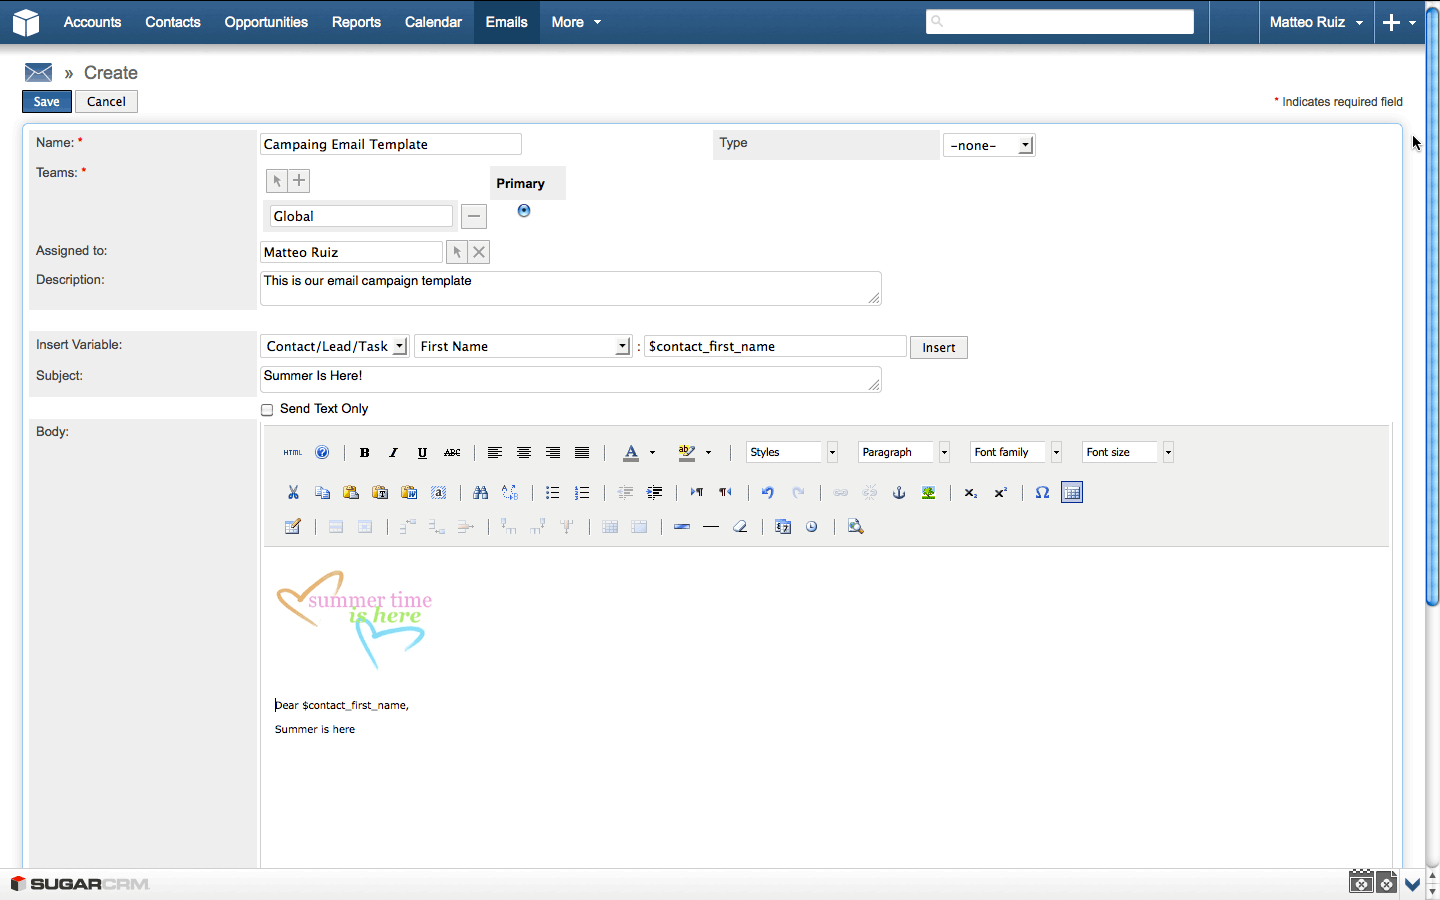
\includegraphics[width=1.00\textwidth]{imgs/SugarCRM-Create_Email.png}
	\caption[SugarCRM Email Composer with Embeded Variables]{SugarCRM Email Composer with Embeded Variables \citep{SugarCRMInc.2013}.}
	\label{fig:SugarCRM-Create_Email}
\end{figure}

Initiated email marketing can be monitored to track response rates, generated leads, and unsubscribed contacts. Marketing target lists also can be imported from third-party lists. SugarCRM also let users save an email as a \ac{HTML} template to use it again within email composer. Finally, it offers a mobile version to let access most of the application features on smartphones and tablet devices \citep{SugarCRMInc.2013}.

\paragraph{Highrise}
Another \ac{SaaS} is Highrise\footnote{http://highrisehq.com/} offering several purchasing plans with 30 days trial period. It has a simple \ac{UI} like SugarCRM, but also provides quick access buttons to add a task or a contact. Task management differentiate it from SugarCRM since there is no calendar view, but a task view in Highrise. These tasks can be synchronized with iCalendar as well. In addition, user can create tasks from emails by using one of the unique email addresses for several time slots provided by Highrise, and adding them into \ac{BCC}, \ac{CC}, or simply simple forwarding an existing email creates a task in Highrise. Contact information can be imported from Outlook or uploading a vCard\footnote{vCard is a file format standard for exchanging business contact information.} file. It provides all the basic contact information fields including the social accounts, however it does not offer custom field creation on those profiles. An email, including its attachments, can also be linked to a contact profile by simply forwarding it to the provided unique email address. If a user does not exist in Highrise when an email from him/her forwarded to link, a contact profile is created using available information in that email. Adding tags to the contact profiles also makes it easier to organize contacts and browsing in them. Highrise does not offer any email composer to do email marketing as in SugarCRM. Therefore, user will depend another product to do simple campaigns. Provided activity view helps users to keep track of their or other users' recent actions within Highrise. Lastly, it offers options to customize the look and feel of the application by provided color schemes.

\subsection{Help Desk Applications}
\label{subsec:3.3.2:HelpDeskAppl}


\paragraph{Zendesk}
Cloud-based customer service software Zendesk \footnote{http://www.zendesk.com} provides a nice and clean \ac{UI}. Zendesk has more than 30,000 businesses from a wide variety of industries. Zendesk offers one-on-one support via many different communication channel including website, email, phone, and social platforms like Facebook and Twitter. Hence, support request coming from those platforms can be turned in to a support ticket. Those support tickets can be group under categories, and more further classification can be done via tags for each ticket. Those feature also help to find related archived resolved tickets, so they can be reused for new tickets. Thanks to the automated process coming with macros a combination of actions can be done with one click like setting status, priority, type of a ticket, and assign it to another person with a predefined comment for the ticket. A ticket can be merged with another one, or copied to the forum to make it available to public, which helps to create a knowledge base. Customer ticket history and basic personal information are kept in the system. However, it does not support to add additional fields to customers' profiles. In addition to desktop version of Zendesk, it support mobile devices as well. Therefore, support team has no dependency on a device. Lastly, provided analytics view by reports give an overview of customer satisfaction and performance of the support team \citep{Zendesk2013,Zendesk2013a}.

\paragraph{Kayako}
Kayako's\footnote{http://www.kayako.com/} complete solution for customer support is named as Kayako Fusion. It comes as software and \ac{SaaS}. Comparing with Zendesk, its \ac{UI} seems more complicated. Kayako has been had more than 30,000 clients since ten years. Kayako does not have social platforms integration like Zendesk, therefore support tickets are generated over website, email, and phone. Tickets can have custom types, statuses, priorities, and tags. Similar to Zendesk, it also supports macros to assign tickets into a department, owner, type, priority, and provide canned responses for tickets with a click. Kayako also keeps basic customer information if they are registered to the system. Registered customers can also support to build a knowledge base in a forum-like environment by contributing others questions a long with support team. Kayako does not have any native app for mobile platforms like Zendesk. Finally, it has a analytics view to keep track of tickets report measuring customer satisfaction and support team performance \citep{KayakoInc.2013,KayakoInc.2013a}.

\subsection{Email Marketing Applications}
\label{subsec:3.1.3:EmaiMarktAppl}


\paragraph{MailChimp}

\paragraph{Constant Contact}



\begin{comment}
--> At the end, put the all the comparison tables together to the Appendix
--> These features are also helped us to add them into our app, decided by saying they all support so we can also support
--> HDesk provides reusibility of emails, CRM provides contact details to replace in email content
\end{comment}
